% CAPITULO 1-------------------------------------------------------------------

\chapter{DESENVOLVIMENTO}
\section{ANÁLISE ORIENTADA À OBJETOS}
\label{sec:desenvolvimento}

Durante o ciclo de vida de desenvolvimento de software, o desennvolvimento normalmente é dividido em estágios, conceitos absratos, soltos, usados para separar as atividades que ocorrem em cada fase do desenvolvimento.

Muitas vezes, essas etapas podem incluir requerimentos, planejamento, design e assim por diantes.

Na fase de análise do sistema ou análise orientada a objetos do desenvolvimento de software, os requisitos do sistema são determinados, as classes são identificadas e os relacionamentos entre as classes são identificados.
As três técnicas de análise que são usadas em conjunto umas com as outras para análise orientada a objetos são modelagem de objetos, modelagem dinâmica e modelagem funcional.

\textbf{A modelagem de objetos desenvolve a estrutur}a estática do sistema de software em termos de objetos. Ele identifica os objetos, as classes nas quais os objetos podem ser agrupados e os relacionamentos entre os objetos. Também identifica os principais atributos e operações que caracterizam cada classe.

Depois que o comportamento estático do sistema é analisado, seu comportamento em relação ao tempo e às mudanças externas precisa ser examinado. Este é o objetivo da modelagem dinâmica.

A Modelagem Dinâmica pode ser definida como uma maneira de descrever como um objeto individual responde a eventos, sejam eventos internos acionados por outros objetos, ou eventos externos acionados pelo mundo exterior.
Considerando o estudo de caso do Sistema FazenTECH, foi realizada a modelagem da atividade de Análise de Sistemas em uma ferramenta CASE de modelagem, contemplando a UML. 

Levamos em consideração as funcionalidades para realização do processo de criação animal e o planejamento de plantio das diferentes culturas da fazenda.

Para atender o domínio de criação animal e planejamento de plantio do Sistema FazenTECH, apresentaremos a seguir o Modelo de Casos de Uso, o Modelo de Classes e o Diagrama de Máquina de Estados para a classe "Plantio", discorrendo sobre pontos em cada um dos tópicos.

a) Diagrama de Use Case:

O objetivo do diagrama de caso de uso é capturar o aspecto dinâmico de um sistema. No entanto, essa definição é muito genérica para descrever o propósito, visto que outros quatro diagramas (atividade, sequência, colaboração e gráfico de estado) também têm o mesmo propósito. Examinaremos algum propósito específico, que o distinguirá de outros quatro diagramas.

Os diagramas de caso de uso são usados para reunir os requisitos de um sistema, incluindo influências internas e externas. Esses requisitos são principalmente requisitos de design. Portanto, quando um sistema é analisado para reunir suas funcionalidades, os casos de uso são preparados e os atores são identificados.

Quando a tarefa inicial é concluída, os diagramas de caso de uso são modelados para apresentar a visão externa.

\begin{figure}[!htb]
    \centering
    \sbox0{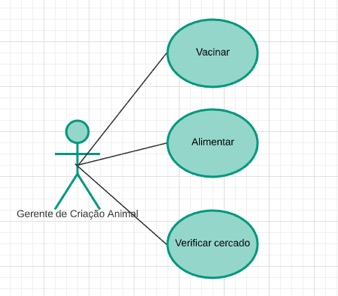
\includegraphics[width=0.5\textwidth]{./dados/figuras/figura1}}% measure width
    \begin{minipage}{\wd0}
    \usebox0
        \caption{Diagrama de Caso de Uso "Criação Animal"}
        \label{fig:figura1}
    \end{minipage}
\end{figure}

\begin{figure}[!htb]
    \centering
    \sbox0{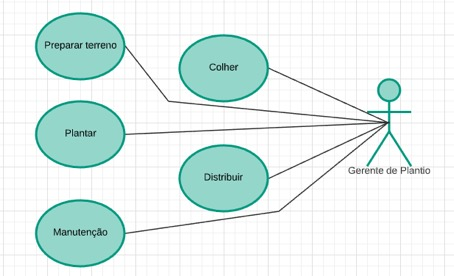
\includegraphics[width=0.5\textwidth]{./dados/figuras/figura2}}% measure width
    \begin{minipage}{\wd0}
    \usebox0
        \caption{Diagrama de Caso de Uso "Plantio"}
        \label{fig:figura2}
    \end{minipage}
\end{figure}

b)	O Modelo de Classe:

 Enquanto o modelo de classes descreve a estrutura dos objetos em um sistema, os diagramas de classes expressam o modelo de classe. O diagrama de classes é um diagrama estático. Ele representa a visão estática de um aplicativo. O diagrama de classes não é usado apenas para visualizar, descrever e documentar diferentes aspectos de um sistema, mas também para construir o código executável do aplicativo de software.
 
O diagrama de classes descreve os atributos e operações de uma classe e também as restrições impostas ao sistema. Os diagramas de classes são amplamente usados na modelagem de sistemas orientados a objetos porque são os únicos diagramas UML, que podem ser mapeados diretamente com linguagens orientadas a objetos.

O diagrama de classes mostra uma coleção de classes, interfaces, associações, colaborações e restrições. Também é conhecido como diagrama estrutural.

\begin{figure}[!htb]
    \centering
    \sbox0{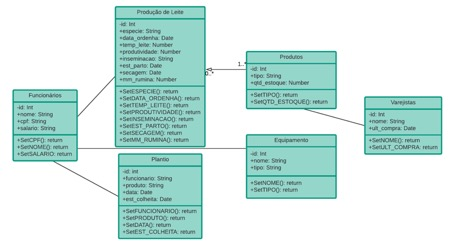
\includegraphics[width=0.5\textwidth]{./dados/figuras/figura3}}% measure width
    \begin{minipage}{\wd0}
    \usebox0
        \caption{Diagrame de Classe}
        \label{fig:figura3}
    \end{minipage}
\end{figure}

c) O Diagrama de Máquina de Estados:

Um diagrama de máquina de estado modela o comportamento de um único objeto, especificando a sequência de eventos pelos quais um objeto passa durante sua vida útil em resposta a eventos. 

O diagrama de máquina de estado é um dos cinco diagramas UML usados para modelar a natureza dinâmica de um sistema. Eles definem diferentes estados de um objeto durante seu tempo de vida e esses estados são alterados por eventos. Os diagramas de máquina de estado são úteis para modelar os sistemas reativos. Os sistemas reativos podem ser definidos como um sistema que responde a eventos externos ou internos.

O diagrama de máquina de estado descreve o fluxo de controle de um estado para outro. Os estados são definidos como uma condição na qual um objeto existe e muda quando algum evento é acionado. O propósito mais importante do diagrama de máquina de estado é modelar o tempo de vida de um objeto desde a criação até o término.

Um estado é denotado por um retângulo arredondado com o nome do estado escrito dentro dele. O estado inicial é denotado por um círculo preto preenchido e pode ser rotulado com um nome. O estado final é denotado por um círculo com um ponto dentro e também pode ser rotulado com um nome.

\begin{figure}[!htb]
    \centering
    \sbox0{
\includegraphics[width=0.5\textwidth]{./dados/figuras/figura4}}% measure width
    \begin{minipage}{\wd0}
    \usebox0
        \caption{Diagrama de Máquina de Estados}
        \label{fig:figura4}
    \end{minipage}
\end{figure}

\section{DESENVOLVIMENTO DE BANCO DE DADOS}

Um banco de dados é um aplicativo separado que armazena uma coleção de dados. Cada banco de dados possui uma ou mais APIs distintas para criar, acessar, gerenciar, pesquisar e replicar os dados que contém.

Outros tipos de armazenamento de dados podem ser usados, como arquivos no sistema de arquivos ou grandes tabelas hash na memória, mas a busca e a gravação de dados não seriam tão rápidas e fáceis com esses tipos de sistemas.

Então, hoje em dia, usamos sistemas de gerenciamento de banco de dados relacional para armazenar e gerenciar um grande volume de dados. Isso é chamado de banco de dados relacional porque todos os dados são armazenados em tabelas diferentes e as relações são estabelecidas usando chaves primárias ou outras chaves conhecidas como chaves estrangeiras.

O sistema FazenTECH precisa armazenar diversas informações importantes e relevantes, como algumas informações pessoas dos usuários, tipos de materiais, fornecedores, produtos, etc.

Existem diversos banco de dados, como o MySQL. MySQL é um sistema de gerenciamento de banco de dados SQL relacional. MySQL é usado dentro da linguagem de programação PHP para fornecer uma interface com bancos de dados MySQL.

Os comandos Data Definition Language (DDL) são usados para criar, manipular e modificar objetos, como usuários, bancos de dados, esquemas, tabelas, visualizações, colunas, funções e procedimentos armazenados. Já os comandos DML são usados para inserir, excluir, atualizar e mesclar dados nas tabelas. Finalmente, os comandos DQL são utilizados para selecionar os registros de uma ou mais tabelas.

Tais comandos também são usados para realizar muitas operações em nível de conta e sessão, como definir parâmetros, inicializar variáveis e iniciar transações.
Isto posto, será demonstrado na sequencia um simples script SQL para auxiliar na criação das tabelas necessárias para o banco de dados "fazenda-bd".

\begin{verbatim}
CREATE DATABASE `fazenda-bd`;

CREATE TABLE `Compras` (
  `id` int(11) NOT NULL,
  `nome` varchar(255) COLLATE utf8_unicode_ci DEFAULT NULL,
  `produto` varchar(255) COLLATE utf8_unicode_ci DEFAULT NULL,
  `qtd` int(11) DEFAULT NULL,
  `dt_compra` date DEFAULT NULL
) ENGINE=InnoDB DEFAULT CHARSET=utf8 COLLATE=utf8_unicode_ci;



INSERT INTO `Compras` (`id`, `nome`, `produto`, `qtd`, `dt_compra`) VALUES
(1, 'Fazenda Sao Francisco', 'sementes de girassol', 900, '2020-08-09'),
(2, 'Comunidade Rural Apaga Fogo', 'sementes de girassol', 1200, '2020-07-14');



CREATE TABLE `Equipamentos` (
  `id` int(11) NOT NULL,
  `nome` varchar(255) COLLATE utf8_unicode_ci DEFAULT NULL,
  `tipo` varchar(255) COLLATE utf8_unicode_ci DEFAULT NULL
) ENGINE=InnoDB DEFAULT CHARSET=utf8 COLLATE=utf8_unicode_ci;



INSERT INTO `Equipamentos` (`id`, `nome`, `tipo`) VALUES
(1, 'colheitadeira', 'motorizado'),
(2, 'ceifadora', 'motorizado');



CREATE TABLE `Funcionarios` (
  `id` int(11) NOT NULL,
  `nome` varchar(255) COLLATE utf8_unicode_ci DEFAULT NULL,
  `cpf` varchar(11) COLLATE utf8_unicode_ci DEFAULT NULL,
  `salario` varchar(15) COLLATE utf8_unicode_ci DEFAULT NULL
) ENGINE=InnoDB DEFAULT CHARSET=utf8 COLLATE=utf8_unicode_ci;



INSERT INTO `Funcionarios` (`id`, `nome`, `cpf`, `salario`) VALUES
(1, 'Roberto Carlos', '53698702134', '1040'),
(2, 'Raul Seixas', '40236902349', '1040'),
(3, 'Elvis Presley', '43749314539', '2650'),
(4, 'Hebert Viana', '33793454294', '2650');



CREATE TABLE `Produc_Leite` (
  `id` int(11) NOT NULL,
  `especie` varchar(255) COLLATE utf8_unicode_ci DEFAULT NULL,
  `data_ordenha` date DEFAULT NULL,
  `temp_leite` int(11) DEFAULT NULL,
  `produtividade` int(11) DEFAULT NULL,
  `inseminacao` varchar(3) COLLATE utf8_unicode_ci DEFAULT NULL,
  `est_parto` date DEFAULT NULL,
  `secagem` date DEFAULT NULL,
  `mm_rumina` int(11) DEFAULT NULL
) ENGINE=InnoDB DEFAULT CHARSET=utf8 COLLATE=utf8_unicode_ci;



INSERT INTO `Produc_Leite` (`id`, `especie`, `data_ordenha`, `temp_leite`, `produtividade`, `inseminacao`, `est_parto`, `secagem`, `mm_rumina`) VALUES
(1, 'marina', '2020-07-13', 33, 1500, 'nao', '2020-09-25', '2021-04-29', 3600),
(2, 'leiteira', '2020-05-22', 39, 2600, 'nao', '2021-02-13', '2021-10-15', 3600);



CREATE TABLE `Produtos` (
  `id` int(11) NOT NULL,
  `nome` varchar(255) COLLATE utf8_unicode_ci NOT NULL,
  `tipo` varchar(255) COLLATE utf8_unicode_ci DEFAULT NULL,
  `qtd_estoque` int(11) DEFAULT NULL,
  `preco` float DEFAULT NULL
) ENGINE=InnoDB DEFAULT CHARSET=utf8 COLLATE=utf8_unicode_ci;



INSERT INTO `Produtos` (`id`, `nome`, `tipo`, `qtd_estoque`, `preco`) VALUES
(1, 'sementes de girassol', 'sementes', 500, 20),
(2, 'enxada', 'material', 300, 70);



CREATE TABLE `Varejistas` (
  `id` int(11) NOT NULL,
  `nome` varchar(255) COLLATE utf8_unicode_ci DEFAULT NULL,
  `ult_compra` date DEFAULT NULL
) ENGINE=InnoDB DEFAULT CHARSET=utf8 COLLATE=utf8_unicode_ci;



INSERT INTO `Varejistas` (`id`, `nome`, `ult_compra`) VALUES
(1, 'Fazenda Sao Francisco', '2020-01-23'),
(2, 'Comunidade Rural Apaga Fogo', '2020-04-15');


ALTER TABLE `Compras`
  ADD PRIMARY KEY (`id`);


ALTER TABLE `Equipamentos`
  ADD PRIMARY KEY (`id`);


ALTER TABLE `Funcionarios`
  ADD PRIMARY KEY (`id`);


ALTER TABLE `Produc_Leite`
  ADD PRIMARY KEY (`id`);


ALTER TABLE `Produtos`
  ADD PRIMARY KEY (`id`);


ALTER TABLE `Varejistas`
  ADD PRIMARY KEY (`id`);


ALTER TABLE `Compras`
  MODIFY `id` int(11) NOT NULL AUTO_INCREMENT, AUTO_INCREMENT=3;


ALTER TABLE `Equipamentos`
  MODIFY `id` int(11) NOT NULL AUTO_INCREMENT, AUTO_INCREMENT=3;


ALTER TABLE `Funcionarios`
  MODIFY `id` int(11) NOT NULL AUTO_INCREMENT, AUTO_INCREMENT=5;


ALTER TABLE `Produc_Leite`
  MODIFY `id` int(11) NOT NULL AUTO_INCREMENT, AUTO_INCREMENT=3;


ALTER TABLE `Produtos`
  MODIFY `id` int(11) NOT NULL AUTO_INCREMENT, AUTO_INCREMENT=3;


ALTER TABLE `Varejistas`
  MODIFY `id` int(11) NOT NULL AUTO_INCREMENT, AUTO_INCREMENT=3;
COMMIT;

SELECT A.nome, B.nome FROM Compras as A INNER JOIN Varejistas as B on A.nome = B.nome;

SELECT COUNT(*) FROM Funcionarios;

SELECT COUNT(DISTINCT nome) FROM Compras;

SELECT MAX(salario) FROM Funcionarios;

\end{verbatim}


\section{LINGUAGENS DE PROGRAMAÇÃO}

Para minimizar as perdas na produção leite que ocorrem na fazenda de Lúcia foi idealizado um sistema de controle de produção utilizando a linguagem Python. A nossa função seria implementar uma busca binária neste sistema.

Python é uma poderosa linguagem de programação de propósito geral. Ele é usado em desenvolvimento web, ciência de dados, criação de protótipos de software e assim por diante. Felizmente para iniciantes, Python tem uma sintaxe simples e fácil de usar. Isso torna o Python uma excelente linguagem para aprender a programar para iniciantes.

Python é uma linguagem de programação de plataforma cruzada, o que significa que pode ser executado em várias plataformas, como Windows, macOS, Linux, e até mesmo foi portado para as máquinas virtuais Java e .NET. É gratuito e de código aberto.
Mesmo que a maioria dos Linux e Mac atuais tenham Python pré-instalado, a versão pode estar desatualizada. Portanto, é sempre uma boa ideia instalar a versão mais atual.

A pesquisa binária é um algoritmo clássico na ciência da computação. Muitas vezes surge em concursos de programação e entrevistas técnicas. Implementar a pesquisa binária acaba sendo uma tarefa desafiadora, mesmo quando é possível entender o conceito. A menos que se esteja curioso ou tenha uma atribuição específica, deve-se sempre aproveitar as bibliotecas existentes para fazer uma pesquisa binária em Python ou qualquer outra linguagem.

A busca binária é um eficiente algoritmo para encontrar um item em uma lista ordenada de itens. Ela funciona dividindo repetidamente pela metade a porção da lista que deve conter o item, até reduzir as localizações possíveis a apenas uma. 
A ideia consiste em basicamente dividir repetidamente uma lista previamente ordenada de vacas leiteiras e aplicarmos a busca binária até encontrarmos as vacas que já foram ordenhadas.   

Exemplo de consulta binária utilizando a linguagem Phyton:


\begin{verbatim}[frame=single]
def busca_binaria(v, p, r, x):
    
      #condição de parada
      if p <= r:
         q = (p+r) // 2  #buscando o índice do meio do vetor
         if x > v[q]:
              return busca_binaria (v, q+1, r, x)
         elif x < v[q]:
              return busca_binaria (v, p, q-1, x)
         else:
              return q #encontrado
      
      return -1  #não encontrado

vacas_ordenhadas = list (range(1,5000))
vaca = 5001
posicao = busca_binaria(vacas_ordenhadas, 0, len(vacas_ordenhadas)-1, vaca)

if posicao >=0:
     print("A vaca %d foi ordenhada e se encontra na posição: %d." % (vaca,posicao))
else:
     print("A vaca NÃO foi ordenhada.")

print (vacas_ordenhadas)
\end{verbatim}

